\documentclass[11pt,a4paper]{report}
\usepackage[left=3cm,right=3cm,top=3cm,bottom=3cm]{geometry}
\usepackage[utf8]{inputenc}
\usepackage[francais]{babel}
\usepackage[T1]{fontenc}
\usepackage{graphicx}
\usepackage{blindtext}
\usepackage{listings}
\usepackage{amsmath}
\usepackage{amssymb}

\makeatletter
\renewcommand{\@chapapp}{Exercice}
\makeatother

%\setlength{\parindent}{0.7cm}
\setlength{\parskip}{\baselineskip}

\begin{document}

\begin{titlepage}

\centering

\includegraphics[scale=0.4]{SU.png}\par\vspace{1cm}
\vspace{1cm}
{\scshape\bfseries ARA\par}
\vspace{1.5cm}
{\huge\bfseries Projet Peersim\par}
\vspace{2cm}
{\Large\itshape Robin Blottiere-Mayo\par
	Pierre Oumeddour\par}
\vfill
{\Large Professeur : Jonathan Lejeune}
\vfill

% Bottom of the page
{\large \today\par}
\end{titlepage}

%\title{ARA}
%\title{Projet Peersim}
%\author{Robin Blottiere-Mayo\\
%	Pierre Oumeddour\\
%	Professeur : Jonathan Lejeune}
%\date{\today}

%\maketitle

\pagenumbering{arabic}

\chapter{}

\section{Question 1 :}

L'algorithme de verrouillage utilisé dans la classe Application est un algorithme dérivé de celui de Naimi-Tréhel utilisant la notion de jeton.
%\linespread{0.5}

Ainsi tous les sites se partagent le même jeton et seul le site possédant le jeton peut entrer en section critique. Dans la classe Application, les constantes initial\_owner et nil servent à discriminer le site possédant le jeton des autres.
%\linespread{1.7}

Chaque noeud maintient sa propre liste de noeuds en attente de section critique (variable next) et son compteur global de sections critiques (variable global\_counter). Il possède également l'adresse du noeud dont il pense qu'il possède le jeton (variable last) ainsi que le nombre de sections critiques qu'il a lui-même effectuées (variable nb\_cs). Si un noeud veut une section critique, il envoie une demande pour avoir le jeton puis il se met en attente.
%\linespread{0.5}

Quand un noeud sort de section critique, il envoie le jeton au dernier noeud de la liste des noeuds demandant la section critique avec les informations qu'il possède du nombre de sections critiques réalisées et des noeuds en attente de section critique.
%\linespread{0.5}

Lorsqu'un noeud reçoit le jeton, il met à jour son compteur de sections critiques avec la valeur envoyée par le dernier noeud ayant été en section critique. Il compare également sa liste de noeuds en attente avec celle qu'il a reçue. Si des noeuds se trouvent dans les deux listes mais pas dans le même ordre, l'ordre envoyé par le dernier noeud en section critique est maintenu. Si des demandes sont absentes de la liste reçue, elles sont ajoutées en fin de liste.


\section{Question 2 :}

On considère trois états du jeton :
\begin{enumerate}
	\item Un noeud possède le jeton mais ne s’en sert pas (état tranquille).
	\item Un noeud possède le jeton et est en section critique (état utilisé).
	\item Le jeton est en transit (état enTransit).
\end{enumerate}

%\lstset{language=C}
%\begin{lstlisting}
tranquille \to utilisé : la section critique est demandée et personne ne requiert le jeton.
tranquille \to enTransit : un noeud requiert le jeton.
utilisé \to tranquille : la section critique se termine.
utilisé \to enTransit : releaseCS(timeout) && !next.isEmpty()
enTransit \to utilisé : receive_token()
%\end{lstlisting}
%\lstset{language=latex}


\section{Question 3 :}

On peut charger des bibliothèques.\\
Application > (OS : File Système, Driver) > Matériel\\
Avantages :\\
Modulable, empreinte mémoire réduite.\\
Inconvénients :\\
Sécurité : tout s’exécute dans le noyau, le noyau est modifiable.\\
Caractéristiques :\\
- Interaction directe avec le matériel,\\
- Modules exécutés en kernel space,\\
- Code optimisé pour une architecture,\\
- Services sous forme de module.

\section{Ex-noyau :}

Ne gère que les interruptions, tout est au niveau user.\\
File Système > Gestionnaire d’interruption > Matériel\\
Caractéristiques :\\
- Interaction directe avec le matériel,\\
- Ensemble des services en user mode,\\
- Gestion de ressources physique au niveau applicatif.

1971 première version UNIX écrit en assembleur.\\
1973 tout UNIX est réécrit en C V4.\\
1974 V5 open source pour les universitaires.\\
1977 V6 étudiée en cours au premier semestre.\\
1978 V7 la licence devient payant.\\
1979 BSD développé à partir de la dernière version libre d’UNIX (V6).\\
1991 Premier Linux\\
1994 premier noyau stable (1.0)\\
1995 Intégration des modules (1.2)\\
2003 le noyau deviens préemptible (2.6)\\
2015 Linux étudié en cours (4.2.3).

Le noyau Linux offre 5 grandes fonctionnalités :\\
1. Gestion des processus,\\
2. Gestion de la mémoire,\\
3. Gestion des services réseaux,\\
4. Gestion du stockage,\\
5. Gestion de l’interface avec l’utilisateur.

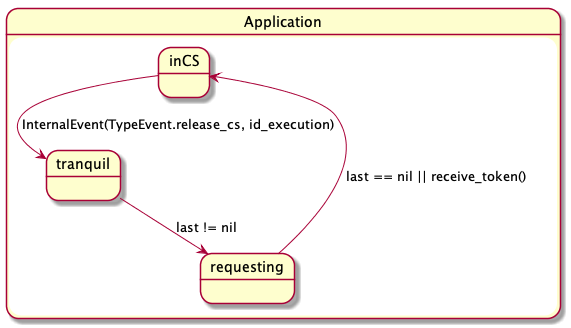
\includegraphics[scale=0.3]{../Diagrammes/exercice_1-question_2.png}


\chapter{}


+ Inline\\
Avantages :\\
- Permet d’économiser le coût d’un appel de fonction.\\
- Permet des optimisations impossible avec un appel.\\
Inconvénient :\\
- Augmente la taille du code, donc les cache miss.\\
- Utilisations accrue des registres pour les paramètres.

Propre à gcc mais pas POSIX :\\
likely(), unlikely(). Fait deux sauts dans le cas le moins probable et 0 dans le cas le plus probable.

asmlinkage : Précède tous les appel système. Force le passage par la pile système.

le struct hack (c’est vraiment très important !).

char oui[4] est une constante symbolique. Il n’y a pas de case d’adresse. Un pointeur de fonction est aussi une constante symbolique.\\
=> \&oui == oui c’est un identificateur de vecteur.

+ La fonction vmalloc() peut être utilisée pour obtenir des zones mémoire continues dans l’espace d’adresse virtuel même si les pages ne sont pas en continues en mémoire physique.

+ La fonction ioremap() ne fait pas d’allocation, mais fait correspondre le segment donné en mémoire physique dans l’espace d’adressage virtuel. 


\chapter{}


\end{document}
